\begin{figure}[t]
    \centering
    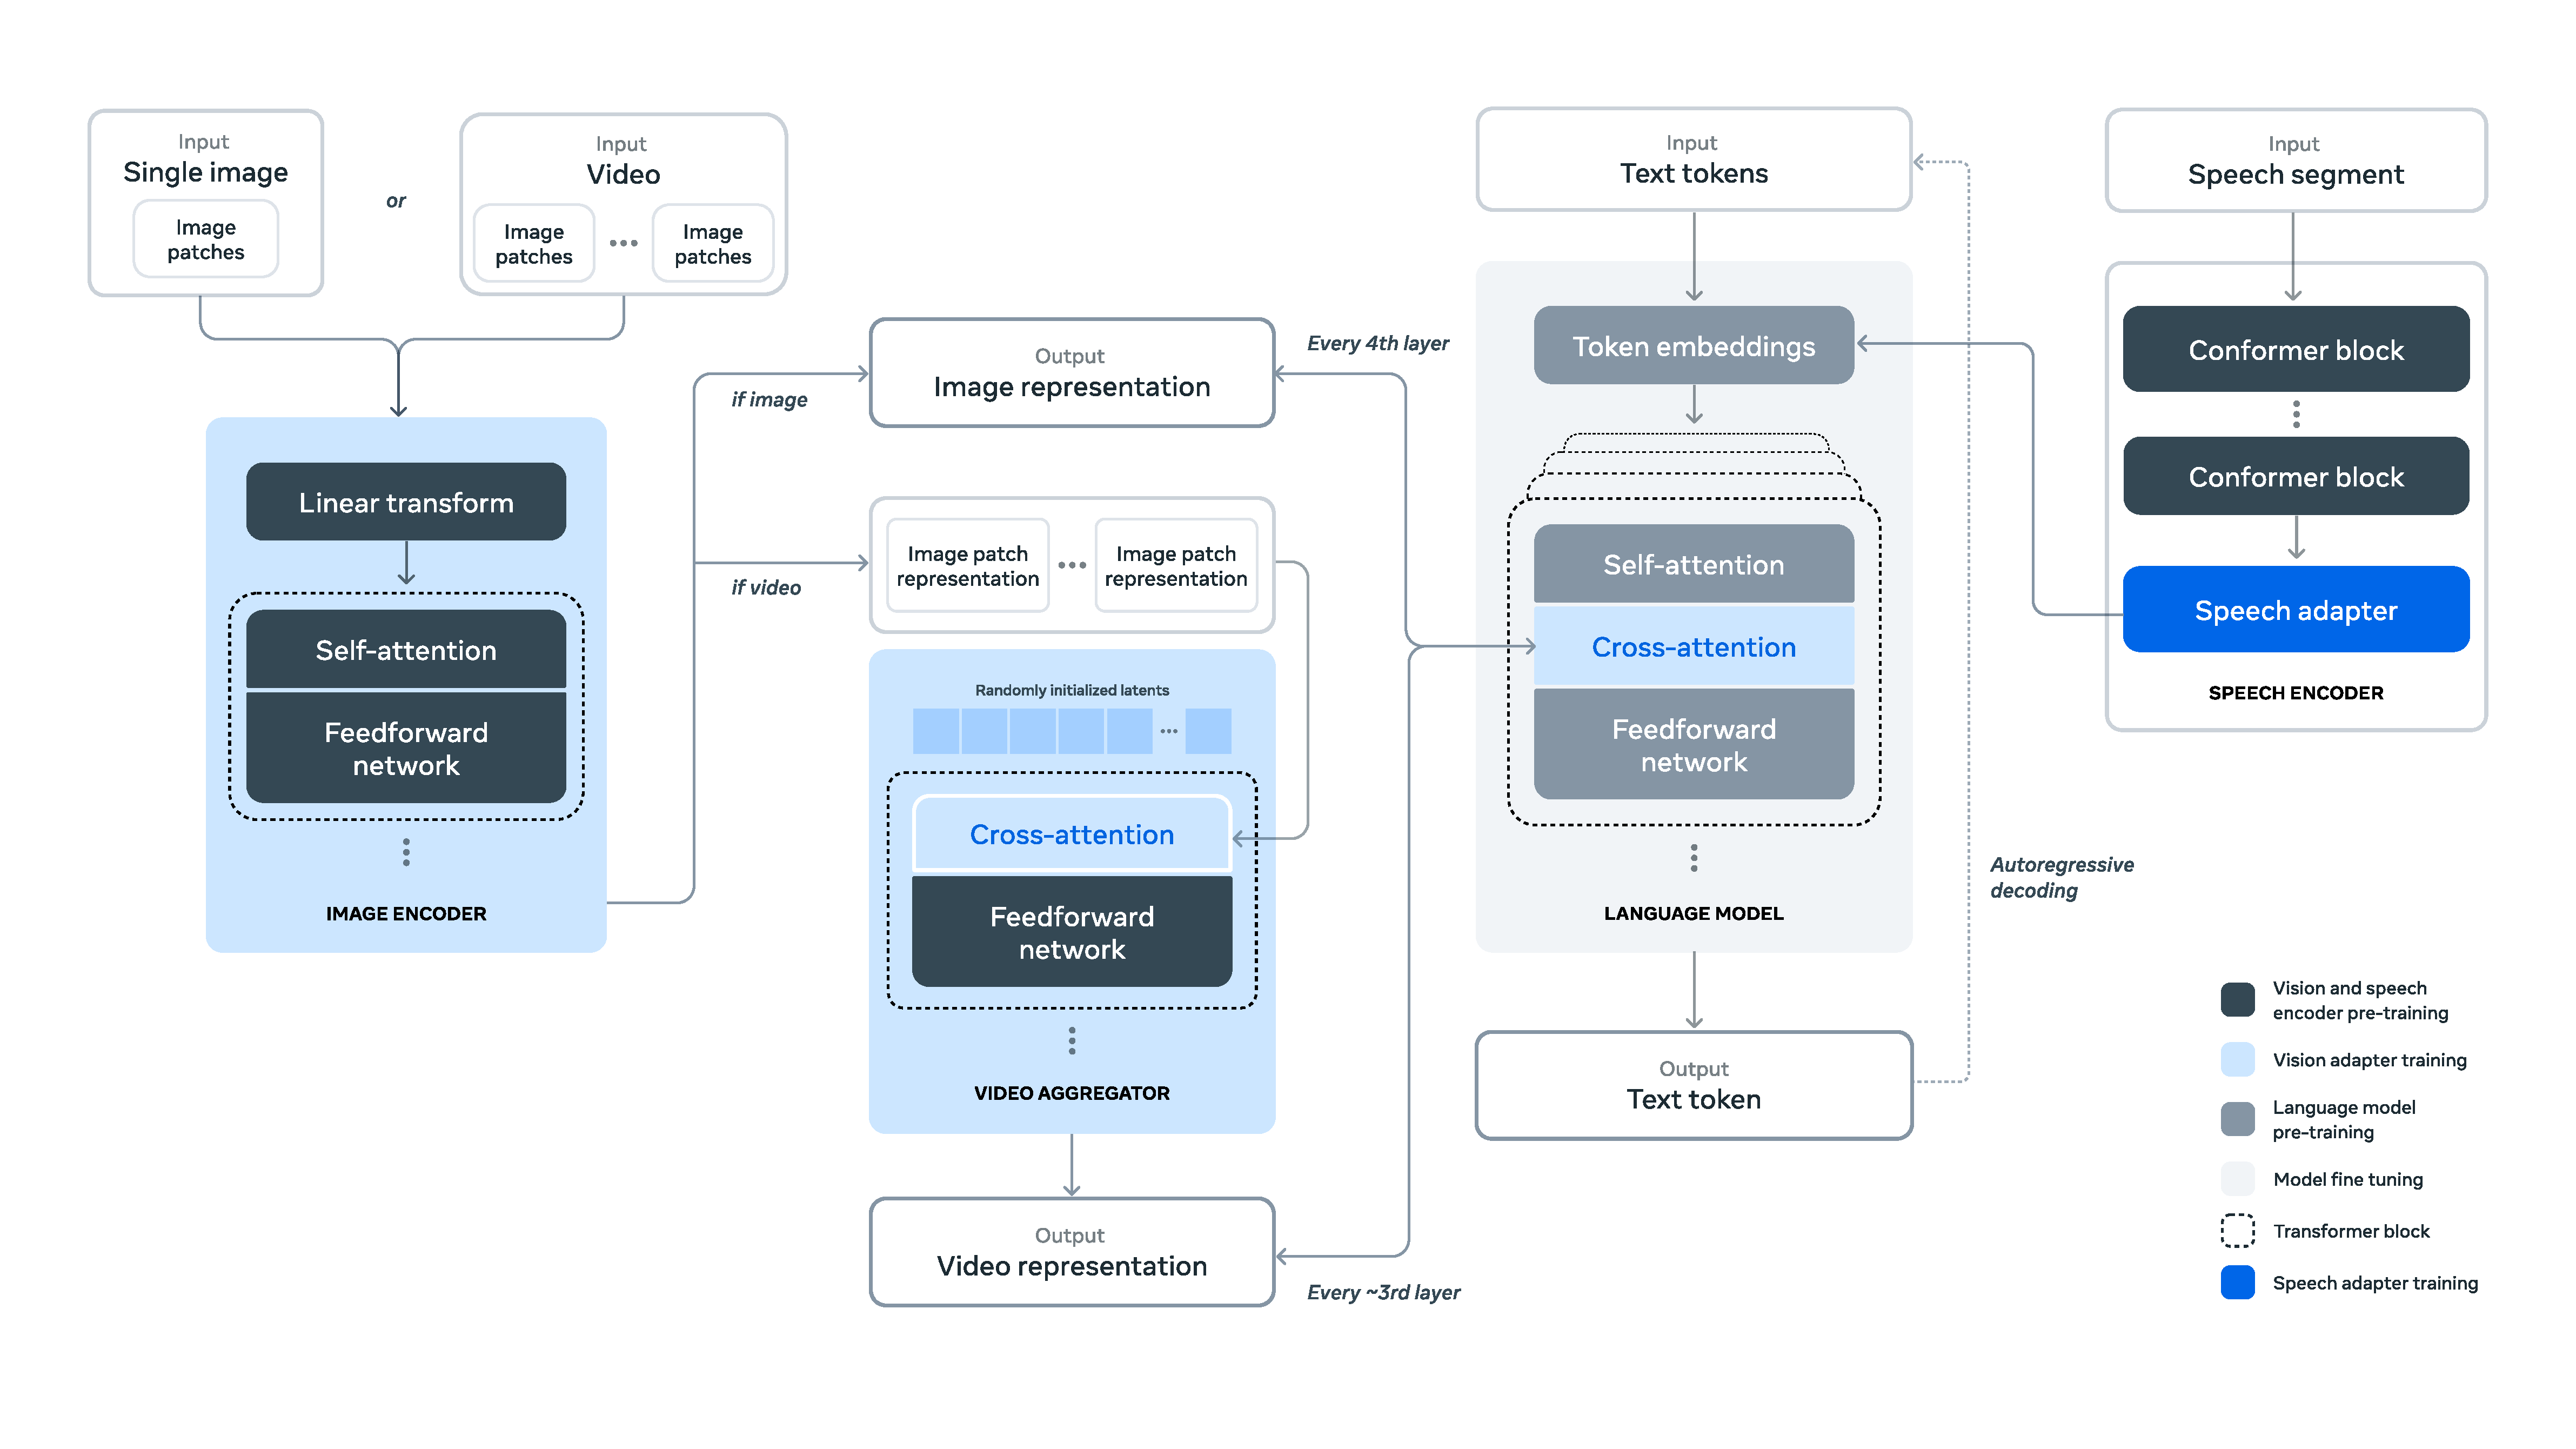
\includegraphics[width=\textwidth]{assets/llama3_architecture.pdf}
    \caption{\textbf{Illustration of the compositional approach to adding multimodal capabilities to Llama 3 that we study in this paper.} This approach leads to a multimodal model that is trained in five stages: \textbf{(1)} language model pre-training, \textbf{(2)} multi-modal encoder pre-training, \textbf{(3)} vision adapter training, \textbf{(4)} model finetuning, and \textbf{(5)} speech adapter training.}
    \label{sph:fig:multimodal_model_overview}
\end{figure}

\section{Vision Experiments}
\label{section:vision}

We perform a series of experiments in which we incorporate visual-recognition capabilities into \llamathree via a compositional approach that consists of two main stages.
First, we compose a pre-trained image encoder \citep{xu2023demystifying} and the pre-trained language model by introducing and training a set of cross-attention layers between the two models \citep{alayrac2022flamingo} on a large number of image-text pairs.
This leads to the model illustrated in Figure~\ref{sph:fig:multimodal_model_overview}.
Second, we introduce temporal aggregator layers and additional video cross-attention layers that operate on a large collection of video-text pairs to learn the model to recognize and process temporal information from videos.

A compositional approach to foundation model development has several advantages: \textbf{(1)} it enables us to parallelize the development of the vision and language modeling capabilities; \textbf{(2)} it circumvents complexities of joint pre-training on visual and language data that stem from tokenization of visual data, differences in background perplexities of tokens originating from different modalities, and contention between modalities; \textbf{(3)} it guarantees that model performance on text-only tasks is not affected by the introduction of visual-recognition capabilities, and \textbf{(4)} the cross-attention architecture ensures that we do not have to expend compute passing full-resolution images through the increasingly LLM backbones (specifically, the feed-forward networks in each transformer layer), making it more efficient during inference.
We note that our multimodal models are still under development and not yet ready for release.

Before presenting the results of our experiments in Section~\ref{section:results_image_recognition} and~\ref{section:results_video_recognition}, we describe the data we used to train visual recognition capabilities, the model architecture of the vision components, how we scale training of those components, and our pre-training and post-training recipes.

% \section{Center Embedding Leads to The Hierarchical Rule}
\section{Data Complexity Determines Rule Preference}
\label{sec:data_complexity}

We find that models generalize hierarchically because they are trained on data which includes center embeddings, a linguistic structure which we describe in Section \ref{sec:center_embed}. Center-embedded sentences drive hierarchical generalization in both the QF task (Section \ref{sec:qf_result}) and the TI task (Section \ref{sec:ti_result}).

\begin{figure}[t!]
    \centering
    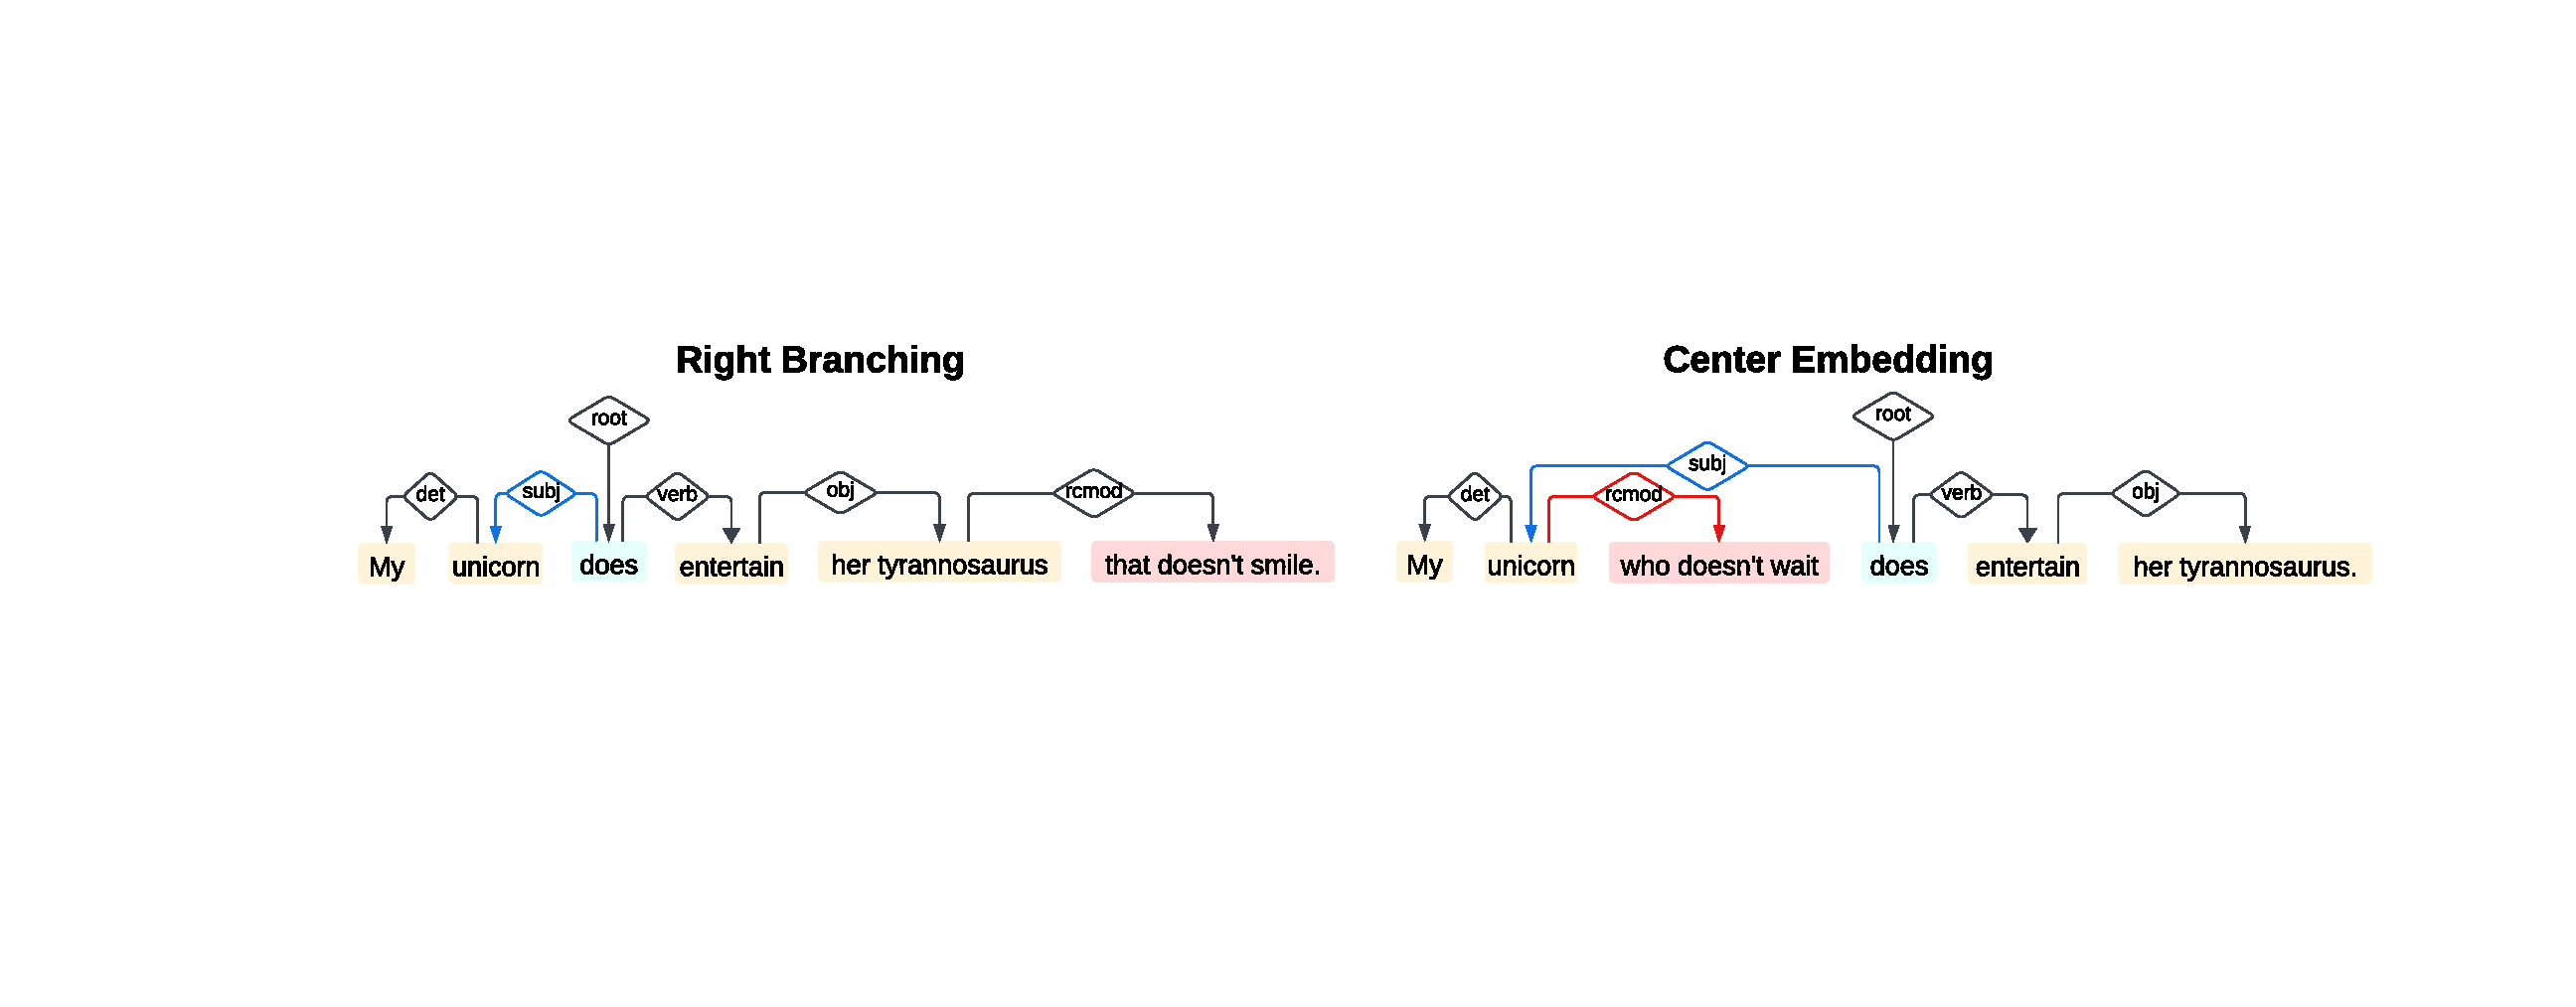
\includegraphics[width=1.0\textwidth]{figures/sentence_demo.pdf}
    \caption{\textbf{Sentence Examples.}   \textit{Left:} Right-branching sentence example. The linear progression of the main constituent is not interrupted by the relative clause. 
    \textit{Right:} Center-embedded sentence example. When the relative clause modifies the subject, it interrupts the linear progression of the main constituent. 
    }
    \label{fig:sentence_demo}
\end{figure}

\subsection{Center Embedding}
\label{sec:center_embed}
Center embedding occurs when a clause is placed recursively within another clause of the same type. Figure \ref{fig:sentence_demo} (\textit{left}) illustrates two examples of center-embedded sentences, where the embedded clause complicates syntactic parsing by placing an additional subject noun in between a verb and its own subject. Whereas center embeddings exhibit a recursive structure, sentences without center embeddings are exclusively right-branching. Right-branching structures may also include modifying clauses, but these clauses can only be appended at the end of the main clause, maintaining its linear flow (see Figure \ref{fig:sentence_demo}, \textit{right}). Linguists have long argued that center embeddings play a crucial role in grammar acquisition \citep{wexler1980formal} and give rise to tree-like syntactic structures \citep{Chomsky2015-bg}. 


We find that center embeddings, which are crucial for human language acquisition, also lead an LM to acquire hierarchical grammar rules. To correctly predict the next token, LMs must track syntactic connections between words in the context. In right-branching sentences, LMs can rely on linear proximity to identify these connections; as shown in Figure \ref{fig:sentence_demo}, a simple bigram model suffices to capture the subject-verb relationship for such sentences. In contrast, center embeddings introduce relative clauses of various lengths, making linear n-gram models inefficient for capturing subject-verb relationships. The recursive nature of the center embedding requires the model to track multiple subject-verb relationships: one for the main clause and a separate one for the embedded relative clause. In these cases, a tree structure is more efficient to model subject-verb relationships. 


\subsection{Question Formation Results}
\label{sec:qf_result}
As specified in Section \ref{sec:qf_task}, the training data for QF is ambiguous between the linear rule (i.e., moving the first auxiliary) and the hierarchical rule (i.e., moving the main auxiliary). Center-embedded sentences do not meet this ambiguity requirement and, therefore, cannot appear in question formation training samples. To ensure the model is exposed to diverse sentence types, \citet{McCoy2018-uv} introduced a secondary task to the QF training dataset: declaration copying. Like question formation, the declaration-copying example starts with a declarative sentence, but instead of transforming it, the model simply repeats it. Since the ambiguity requirement only applies to the primary question formation task, declaration-copying examples can include center embeddings. Concrete examples of both tasks can be found in Appendix \ref{appdx:data_sample}.


We train models on three modifications of the original training data, varying the composition of the declaration-copying subset. 
In \textit{Quest Only}, we remove all declaration-copying examples.
In \textit{Center embed}, we only keep center-embedded examples. In \textit{Right branch}, we only keep right-branching examples. 
Every modified training sets retains all examples of the primary task, question formation.
Every model trained, regardless of its training set composition, reaches 100\% in-distribution validation accuracy; however, the OOD generalization performance, shown in Figure \ref{fig:grokking_selection} (\textit{left}), differs significantly across the modified training sets. 

Our results confirm that declaration copying examples, specifically center embeddings, are essential for inducing hierarchical generalization.
Models trained without any declaration-copying examples fail to achieve an OOD accuracy above 75\%; so do models trained \textit{only} on right-branching  declaration-copying examples. When trained instead \textit{only} on center-embedded declaration-copying examples, models exhibit a strong preference for the hierarchical rule. This evidence suggests that center-embedded sentences direct a model towards the hierarchical rule. 

\begin{figure}[t!]
    \centering
    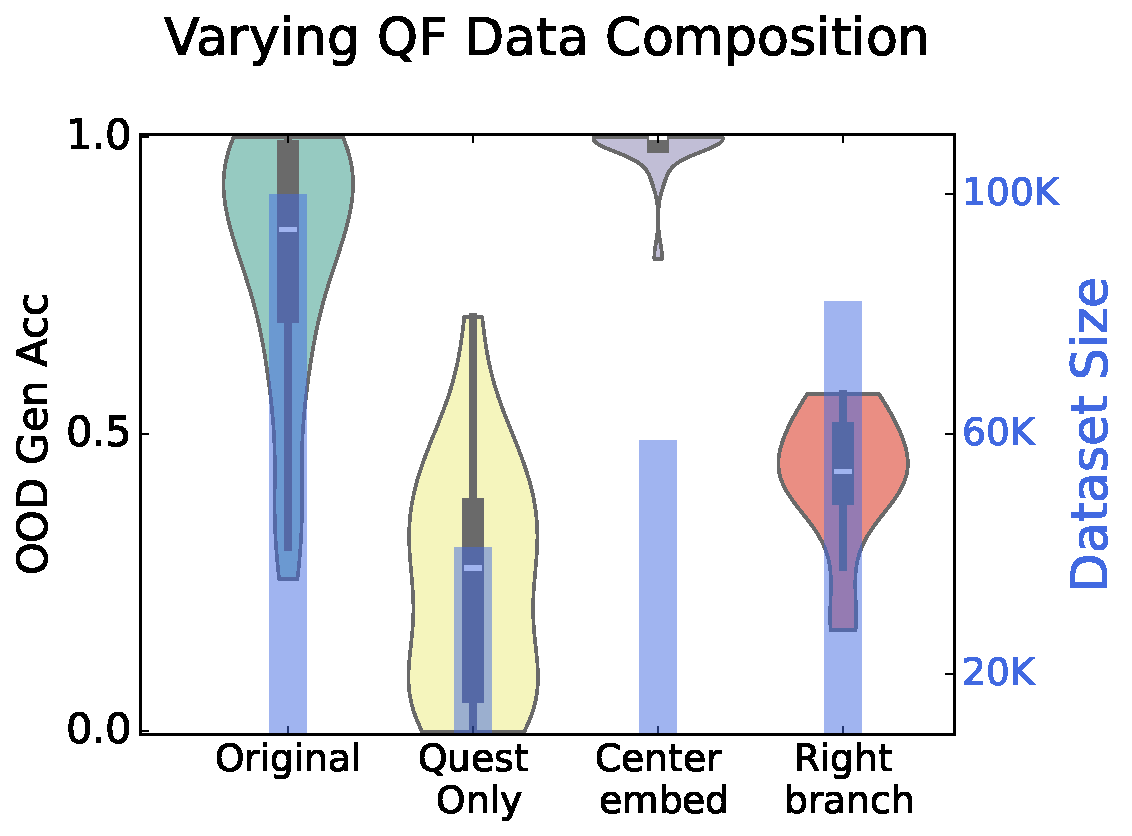
\includegraphics[width=0.41\linewidth]{figures/no_curriculum_main.pdf}
    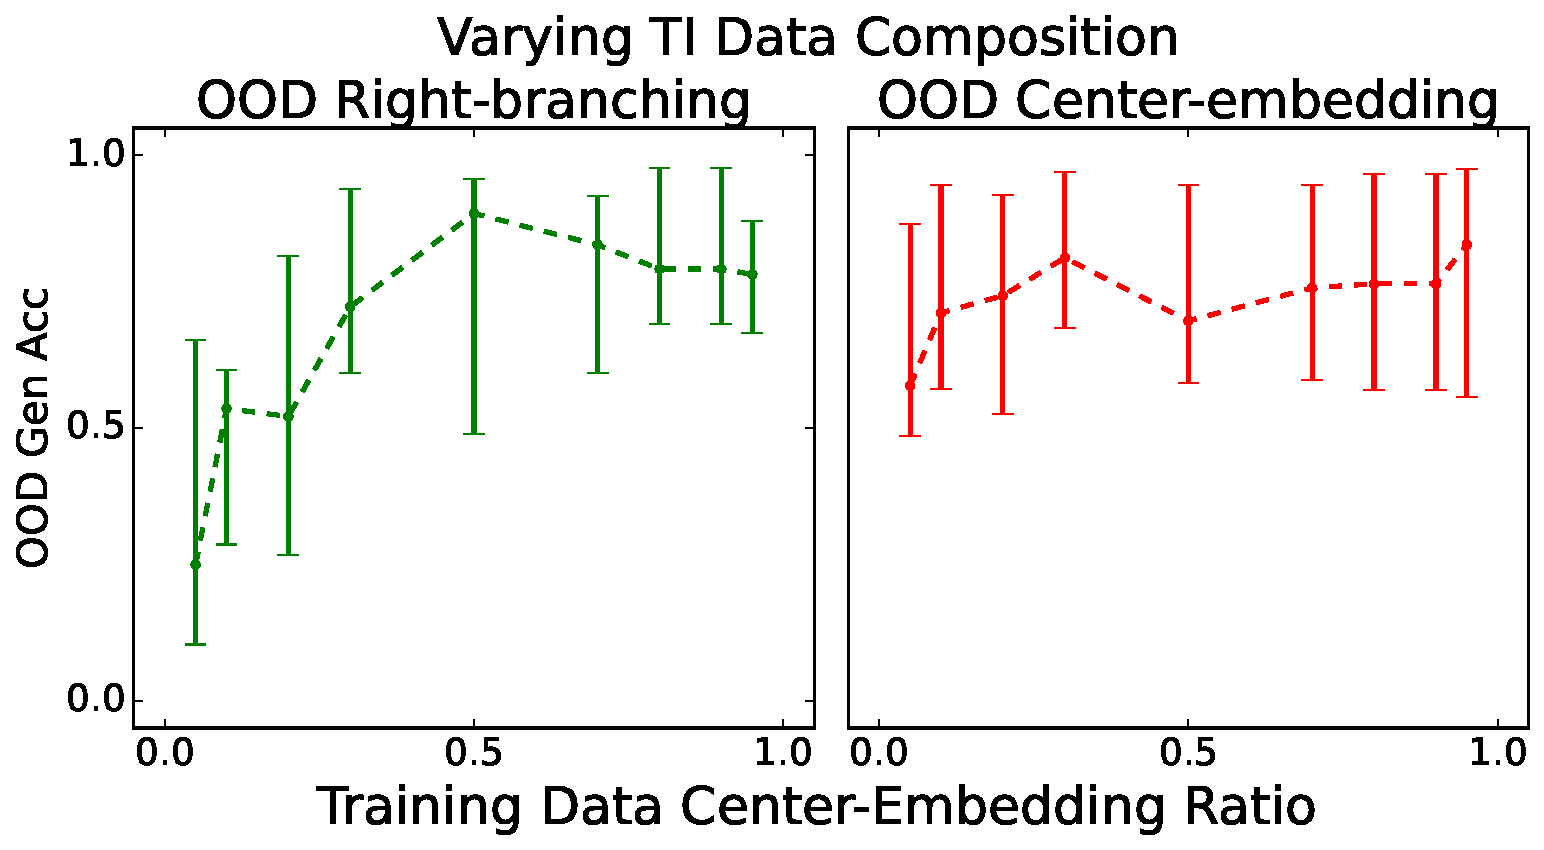
\includegraphics[width=0.55\linewidth]{figures/ti_simplicity_contamination.pdf}
    \caption{
    \textbf{Components of training data drive different generalization behaviors.} 
    \textit{Left:} Center-embedded sentences, which in the QF training data only appear in declaration copying examples, induce hierarchical generalization.
    \textit{Right:} Models are trained on different TI training data mixes and evaluated on two OOD sets: unambiguous right-branching sentences (\textit{green}) and unambiguous center-embedded sentences (\textit{red}). For center-embedded sentences, the hierarchical rule is preferred regardless of data mixes. For right-branching sentences, the model's preference for the hierarchical rule is exclusively driven by having a large mix of center-embedded sentences in the TI training data.}
    \label{fig:grokking_selection}
\end{figure}



\subsection{Tense Inflection Results}
\label{sec:ti_result}

In the TI training data, both right-branching and center-embedded sentences are made ambiguous by ensuring the distractor noun (i.e., a noun that appears between the main subject and the main verb) shares the same plurality as the main subject. For right-branching sentences, the distractor noun occurs in a prepositional phrase. For center-embedded sentences, the distractor noun occurs in a relative clause; either the subject or the object of the modifying clause can act as the distractor noun. We list examples below: 

\begin{enumerate}[itemsep=2pt,labelindent=10pt,topsep=0pt,parsep=0pt,partopsep=1pt, align=left, leftmargin=*]
    \item \textbf{Right Branching}: The noun in the prepositional phrase (e.g., `` \textit{to the cabinet}") acts as the distractor in the TI task.
    
    Example A (ID): \textit{The keys to the \textbf{cabinets} are on the table.}

    Example B (OOD): \textit{The keys to the \textbf{cabinet} are on the table.}
    
    \item \textbf{Center Embedding}: Either the subject or the object inside the relative clause acts as the distractor in the TI task.

    Example C (ID): \textit{The keys that unlock the \textbf{cabinets} are on the table.}

    Example D (OOD): \textit{The keys that unlock the \textbf{cabinet} are on the table.}
    
    
\end{enumerate}
We create variations of the TI training data by adjusting the ratio of right-branching to center-embedded samples while keeping the total training size constant.\footnote{The original training dataset contains a secondary past-tense copying task, to parallel the declaration-copying secondary task in QF. We show in Appendix \ref{appdx:ti_secondary} that the secondary task is not necessary, and we do not include it in our modified training sets.} A model's generalization behavior is tested on two OOD sets: one containing unambiguous right-branching sentences (e.g., Example B) and the other containing unambiguous center-embedded sentences (e.g., Example D). 

Generalization accuracies are shown in Figure \ref{fig:grokking_selection} (\textit{right}). When the training data is dominated by ambiguous right-branching sentences, the model fails to learn the hierarchical rule, as indicated by low OOD accuracy. However, when trained on a greater proportion of center-embedded sentences, the model systematically applies the hierarchical rule to both right-branching and center-embedded OOD sentences. As shown in Figure \ref{fig:grokking_selection} (\textit{right}), regardless of its training data mix, the model  generalizes hierarchically to OOD \textit{center embeddings}. In contrast, the model only generalizes hierarchically to \textit{right-branching sentences} after being exposed to a sufficient quantity of center-embedded sentences during training. In other words, the model eventually learns to treat non-recursive sequences as hierarchical through exposure to recursive center embeddings. These observations suggest that center embeddings drive the model's overall preference for tree structures. For further analysis of which center embedding structures induce this bias most efficiently, see Appendix \ref{appdx:obj_sbj_ctr_breakdown}.

% %%%%%%%%%%%%%%%%Previous version to preserve comments %%%%%%%%%%%%%%%%%%%%%%%%%%%%%%%%%%%%%%%%
% \iffalse
% \subsection{Tense Inflection} 
% \label{sec:ti_result}
% We now analyze hierarchical generalization in the tense inflection task, demonstrating the generality of our findings across grammatical rules. 
% The tense inflection setting from \citet{Linzen2016-vx} uses the same generation process as the question formation task, changing only the task itself.  
% This generation process leads to three types of sentences:

% \begin{enumerate}[itemsep=2pt,labelindent=10pt,topsep=0pt,parsep=0pt,partopsep=1pt, align=left, leftmargin=*]
%     \item The main verb immediately follows the subject noun.

%     Example: \textit{The keys are on the table.}
%     \item The main verb and the subject noun are separated by a prepositional phrase (e.g., `` \textit{to the cabinet}"). In all sentence examples, the prepositional phrase consistently follows the same syntactical structure and length (i.e., ``preposition $+$ determiner $+$ noun"). 

%     Example: \textit{The keys to the cabinet are on the table.}
%     \item The main verb and subject noun are separated by a relative clause, which can vary in syntactic composition and length.

%     Example: \textit{The keys that I used to unlock the cabinet are on the table.}
% \end{enumerate}


% By definition, both the first and second sentence types are right branching. In the second type, although a prepositional phrase is inserted within the main clause, it differs syntactically from a relative clause modifier. Unlike relative clause modifiers, prepositional phrases lack syntactic diversity, whereas relative clauses can exhibit the same of diversity as an entire sentence. In QF and TI data generated by CFG rules, a 4-gram model suffices to capture the subject-verb agreement. In contrast, relative clause modifiers (i.e., the third type) vary in both length and syntactic structure. All three sentence types are present in the original training data. Since sentences of the first type lack a distractor noun, they cannot be used to probe the model’s generalization, so the generalization set includes only the second and third types. As specified in Section \ref{sec:ti_task}, the TI training data only requires that the subject and distractor have the same plurality. Thus, center-embedded sentences can be included in the TI training data without violating the ambiguity requirement, and a secondary task is not necessary for TI.\footnote{In Appendix \ref{appdx:tense_tv}, we show that we can again leverage a secondary task such that a model trained on center-embedded tense inflection examples can generalize to right-branching sentences without having seen any examples of tense inflection on the sentence type, but not vice versa. }


% Our goal is to verify that center embeddings also drive OOD generalization in tense inflection. We create variations of the TI training data by adjusting the ratio of right-branching to center-embedded sentences, keeping the total training size constant. In Figure \ref{fig:ti_selection}, we report the model's OOD behavior across two data partitions. Figure \ref{fig:ti_selection} (\textit{left}) shows the model's generalization accuracy on unambiguous right-branching sentences when trained on different data mixes. When training data is dominated by ambiguous right-branching sentences, the model fails to learn the hierarchical rule, as indicated by low OOD generalization accuracy. However, as we increase the proportion of center-embedded sentences, these sentences---despite being ambiguous---bias the model towards the hierarchical rule, reflected by improved generalization accuracy.

% Figure \ref{fig:ti_selection} (\textit{right}) shows that the model consistently prefers the hierarchical rule for center-embedded sentences, regardless of data composition. These results indicate that the model’s preference for the hierarchical rule is primarily driven by center-embedded sentences. Moreover, with a high proportion of center-embedded sentences in the training data, this hierarchical rule preference extends to right-branching sentences as well.


% \fi
\subsection{Model Architecture}
\label{section:vision_model_architecture}
Our visual-recognition model consists of three main components: \textbf{(1)} an image encoder, \textbf{(2)} an image adapter, and \textbf{(3)} a video adapter.

\textbf{Image encoder.} Our image encoder is a standard vision transformer (ViT; \citet{dosovitskiy2020vit}) that is trained to align images and text \citep{xu2023demystifying}.
We use the ViT-H/14 variant of the image encoder, which has 630M parameters that were trained on 2.5B image-text pairs for five epochs.
The image encoder is pre-trained on images with resolution $224 \times 224$; images were split up into $16 \times 16$ patches of equal size (\emph{i.e.}, a patch size of $14x14$ pixels).
As also demonstrated by prior work such as ViP-Llava \citep{cai2023vipllava}, we observe that image encoders trained via a contrastive text alignment objective are unable to preserve fine-grained localization information. To alleviate this, we employ a \emph{multi-layer} feature extraction, where features from the \emph{4$^{th}$, 8$^{th}$, 16$^{th}$, 24$^{th}$ and 31$^{st}$} layers are also provided in addition to the final layer features.
In addition, we further insert 8 \emph{gated} self-attention layers (making a total of 40 transformer blocks) prior to pre-training of the cross-attention layers to learn alignment-specific features. The image encoder therefore eventually has a total $850$M parameters with the additional layers.
With the multi-layer features, the image encoder produces a $7680$-dimensional representation for each of the resulting $16 \times 16\!=\!256$ patches.
The parameters of the image encoder are \emph{not} frozen during subsequent training stages as we found it to improve performance, especially in domains such as text recognition.

\textbf{Image adapter.} We introduce cross-attention layers between the visual token representations produced by the image encoder and the token representations produced by the language model \citep{alayrac2022flamingo}.
The cross-attention layers are applied after every fourth self-attention layer in the core language model.
Like the language model itself, the cross-attention layers use generalized query attention (GQA) for increased efficiency.
The cross-attention layers introduce substantial numbers of additional trainable parameters into the model: for Llama 3 405B, the cross-attention layers have $\approx$100B parameters.
We pre-train our image adapter in two stages: (1) initial pre-training followed by (2) annealing:
\begin{itemize}
\item \textbf{Initial pre-training.} We pre-train our image adapter on our dataset of  $\sim$6B image-text pairs described above.
For compute efficiency reasons, we resize all images to fit within \emph{at most} four tiles of $336 \times 336$ pixels each, where we arrange the tiles to support different aspect ratios, \emph{e.g.}, $672 \times 672$, $672 \times 336$, and $1344 \times 336$.

\item \textbf{Annealing.}
We continue training the image adapter on $\sim$500M images from the annealing dataset described above.
During annealing, we increase the per-tile image resolution to improve performance on tasks that require higher-resolution images, for example, infographics understanding.
\end{itemize}

\textbf{Video adapter.} Our model takes as input up to 64 frames (uniformly sampled from a full video), each of which is processed by the image encoder.
We model temporal structure in videos through two components: \textbf{(i)} encoded video frames are aggregated by a temporal aggregator which merges 32 consecutive frames into one, \textbf{(ii)} additional video cross attention layers are added before every fourth image cross attention layer.
The temporal aggregator is implemented as a perceiver resampler~\citep{jaegle2021perceiver,alayrac2022flamingo}.
We pre-train using 16 frames per video (aggregated to 1 frame), but increase the number of input frames to 64 during supervised finetuning.
The video aggregator and cross attention layers have 0.6B and 4.6B parameters for Llama 3 7B and 70B, respectively. 




\newcommand{\cq}[1]{\textcolor{red}{\{CQ: #1\}}} %

\subsection{Infrastructure, Scaling, and Efficiency}
\label{section:pretraining_model_scaling}
We describe our hardware and infrastructure that powered \llamathree 405B pre-training at scale and discuss several optimizations that leads to improvements in training efficiency.

\subsubsection{Training Infrastructure}
The Llama 1 and 2 models were trained on Meta's AI Research SuperCluster~\citep{Lee22RSC}. As we scaled further, the training for Llama 3 was migrated to Meta's production clusters~\citep{lee2024building}.%
This setup optimizes for production-grade reliability, which is essential as we scale up training.

\textbf{Compute.}
\llamathree 405B is trained on up to 16K H100 GPUs, each running at 700W TDP with 80GB HBM3, using Meta's Grand Teton AI server platform~\citep{various2022grandteton}. Each server is equipped with eight GPUs and two CPUs. Within a server, the eight GPUs are connected via NVLink. Training jobs are scheduled using MAST~\citep{choudhury2024mast}, Meta's global-scale training scheduler.

\textbf{Storage.} 
Tectonic~\citep{pan2021tectonicfs}, Meta's general-purpose distributed file system, is used to build a storage fabric~\citep{battey2024storage} for Llama 3 pre-training. It offers 240 PB of storage out of 7,500 servers equipped with SSDs, and supports a sustainable throughput of 2 TB/s and a peak throughput of 7 TB/s. A major challenge is supporting the highly bursty checkpoint writes that saturate the storage fabric for short durations. Checkpointing saves each GPU’s model state, ranging from 1 MB to 4 GB per GPU, for recovery and debugging. We aim to minimize GPU pause time during checkpointing and increase checkpoint frequency to reduce the amount of lost work after a recovery. 

\textbf{Network.}
Llama 3 405B used RDMA over Converged Ethernet (RoCE) fabric based on the Arista 7800 and Minipack2 Open Compute Project\footnote{Open Compute Project: \url{https://www.opencompute.org/}} OCP rack switches. Smaller models in the Llama 3 family were trained using Nvidia Quantum2 Infiniband fabric. Both RoCE and Infiniband clusters leverage 400 Gbps interconnects between GPUs.  Despite the underlying network technology differences between these clusters, we tune both of them to provide equivalent performance for these large training workloads. We elaborate further on our RoCE network since we fully own its design.
\begin{itemize}

    \item \textbf{Network topology.} Our RoCE-based AI cluster comprises 24K GPUs\footnote{Note that we use only up to 16K of these 24K GPUs for Llama 3 pre-training.} connected by a three-layer Clos network~\citep{lee2024building}. At the bottom layer, each rack hosts 16 GPUs split between two servers and connected by a single Minipack2 top-of-the-rack (ToR) switch. In the middle layer, 192 such racks are connected by Cluster Switches to form a pod of 3,072 GPUs with full bisection bandwidth, ensuring no oversubscription. At the top layer, eight such pods within the same datacenter building are connected via Aggregation Switches to form a cluster of 24K GPUs. However, network connectivity at the aggregation layer does not maintain full bisection bandwidth and instead has an oversubscription ratio of 1:7. Our model parallelism methods (see Section~\ref{section:4D-parallelism}) and training job scheduler~\citep{choudhury2024mast} are all optimized to be aware of network topology, aiming to minimize network communication across pods.
    
    \item \textbf{Load balancing.} LLM training produces fat network flows that are hard to load balance across all available network paths using traditional methods such as Equal-Cost Multi-Path (ECMP) routing. To address this challenge, we employ two techniques. First, our collective library creates 16 network flows between two GPUs, instead of just one, thereby reducing the traffic per flow and providing more flows for load balancing. Second, our Enhanced-ECMP (E-ECMP) protocol effectively balances these 16 flows across different network paths by hashing on additional fields in the RoCE header of packets.
    
    \item \textbf{Congestion control.} We use deep-buffer switches in the spine~\citep{gangidi2024rmda} to accommodate transient congestion and buffering caused by collective communication patterns. This setup helps limit the impact of persistent congestion and network back pressure caused by slow servers, which is common in  training. Finally, better load balancing through E-ECMP significantly reduces the chance of congestion. With these optimizations, we successfully run a 24K GPU cluster without traditional congestion control methods such as Data Center Quantized Congestion Notification (DCQCN). 
\end{itemize}


\subsubsection{Parallelism for Model Scaling}
\label{section:4D-parallelism}

To scale training for our largest models, we use 4D parallelism—a combination of four different types of parallelism methods—to shard the model. This approach efficiently distributes computation across many GPUs and ensures each GPU's model parameters, optimizer states, gradients, and activations fit in its HBM. Our implementation of 4D parallelism is illustrated in Figure~\ref{fig:4d_parallelism}. It combines tensor parallelism (TP; \citet{NIPS2012_c399862d, shoeybi2019megatron, korthikanti2023reducing}), pipeline parallelism (PP; \citet{huang2019gpipe, narayanan2021efficient, lamy2023breadth}), context parallelism (CP; \citet{liu2023ring}), and data parallelism (DP; \citet{rajbhandari2020zeromemoryoptimizationstraining, ren2021zerooffloaddemocratizingbillionscalemodel, zhao2023pytorch}).

Tensor parallelism splits individual weight tensors into multiple chunks on different devices. Pipeline parallelism partitions the model vertically into stages by layers, so that different devices can process in parallel different stages of the full model pipeline. Context parallelism divides the input context into segments, reducing memory bottleneck for very long sequence length inputs. We use fully sharded data parallelism \citep[FSDP;][]{rajbhandari2020zeromemoryoptimizationstraining, ren2021zerooffloaddemocratizingbillionscalemodel, zhao2023pytorch}, which shards the model, optimizer, and gradients while implementing data parallelism which processes data in parallel on multiple GPUs and synchronizes after each training step. Our use of FSDP for Llama 3 shards optimizer states and gradients, but for model shards we do not reshard after forward computation to avoid an extra \texttt{all-gather} communication during backward passes.

\textbf{GPU utilization.}
Through careful tuning of the parallelism configuration, hardware, and software, we achieve an overall BF16 Model FLOPs Utilization (MFU; \citet{chowdhery2023palm}) of 38-43\% for the configurations shown in Table~\ref{table:mfu}.  The slight drop in MFU to 41\% on 16K GPUs with DP=128 compared to 43\% on 8K GPUs with DP=64 is due to the lower batch size per DP group needed to keep the global tokens per batch constant during training.

\begin{table}
	\centering
	\begin{tabular}{cccccccc|cc}
	\toprule
	     \textbf{GPUs} & \textbf{TP} & \textbf{CP} & \textbf{PP} & \textbf{DP}   & \textbf{Seq. Len.} &   \textbf{Batch size/DP} & \textbf{Tokens/Batch} & \textbf{TFLOPs/GPU} & \textbf{BF16 MFU}\\ 
	\midrule
	8,192    & 8 & 1 & 16 & 64   & 8,192   &   32 & 16M  & 430      & 43\%        \\
	16,384   & 8 & 1 & 16 & 128   & 8,192   &   16 & 16M  & 400      & 41\%        \\
	16,384   & 8 & 16 & 16 & 8   & 131,072 &   16 & 16M   & 380     & 38\%        \\
	\bottomrule

	\end{tabular}
\caption{\textbf{Scaling configurations and MFU for each stage of \llamathree 405B pre-training.} See text and Figure \ref{fig:4d_parallelism} for descriptions of each type of parallelism.}
\label{table:mfu}
\end{table}

\begin{figure}[t]
     \centering
     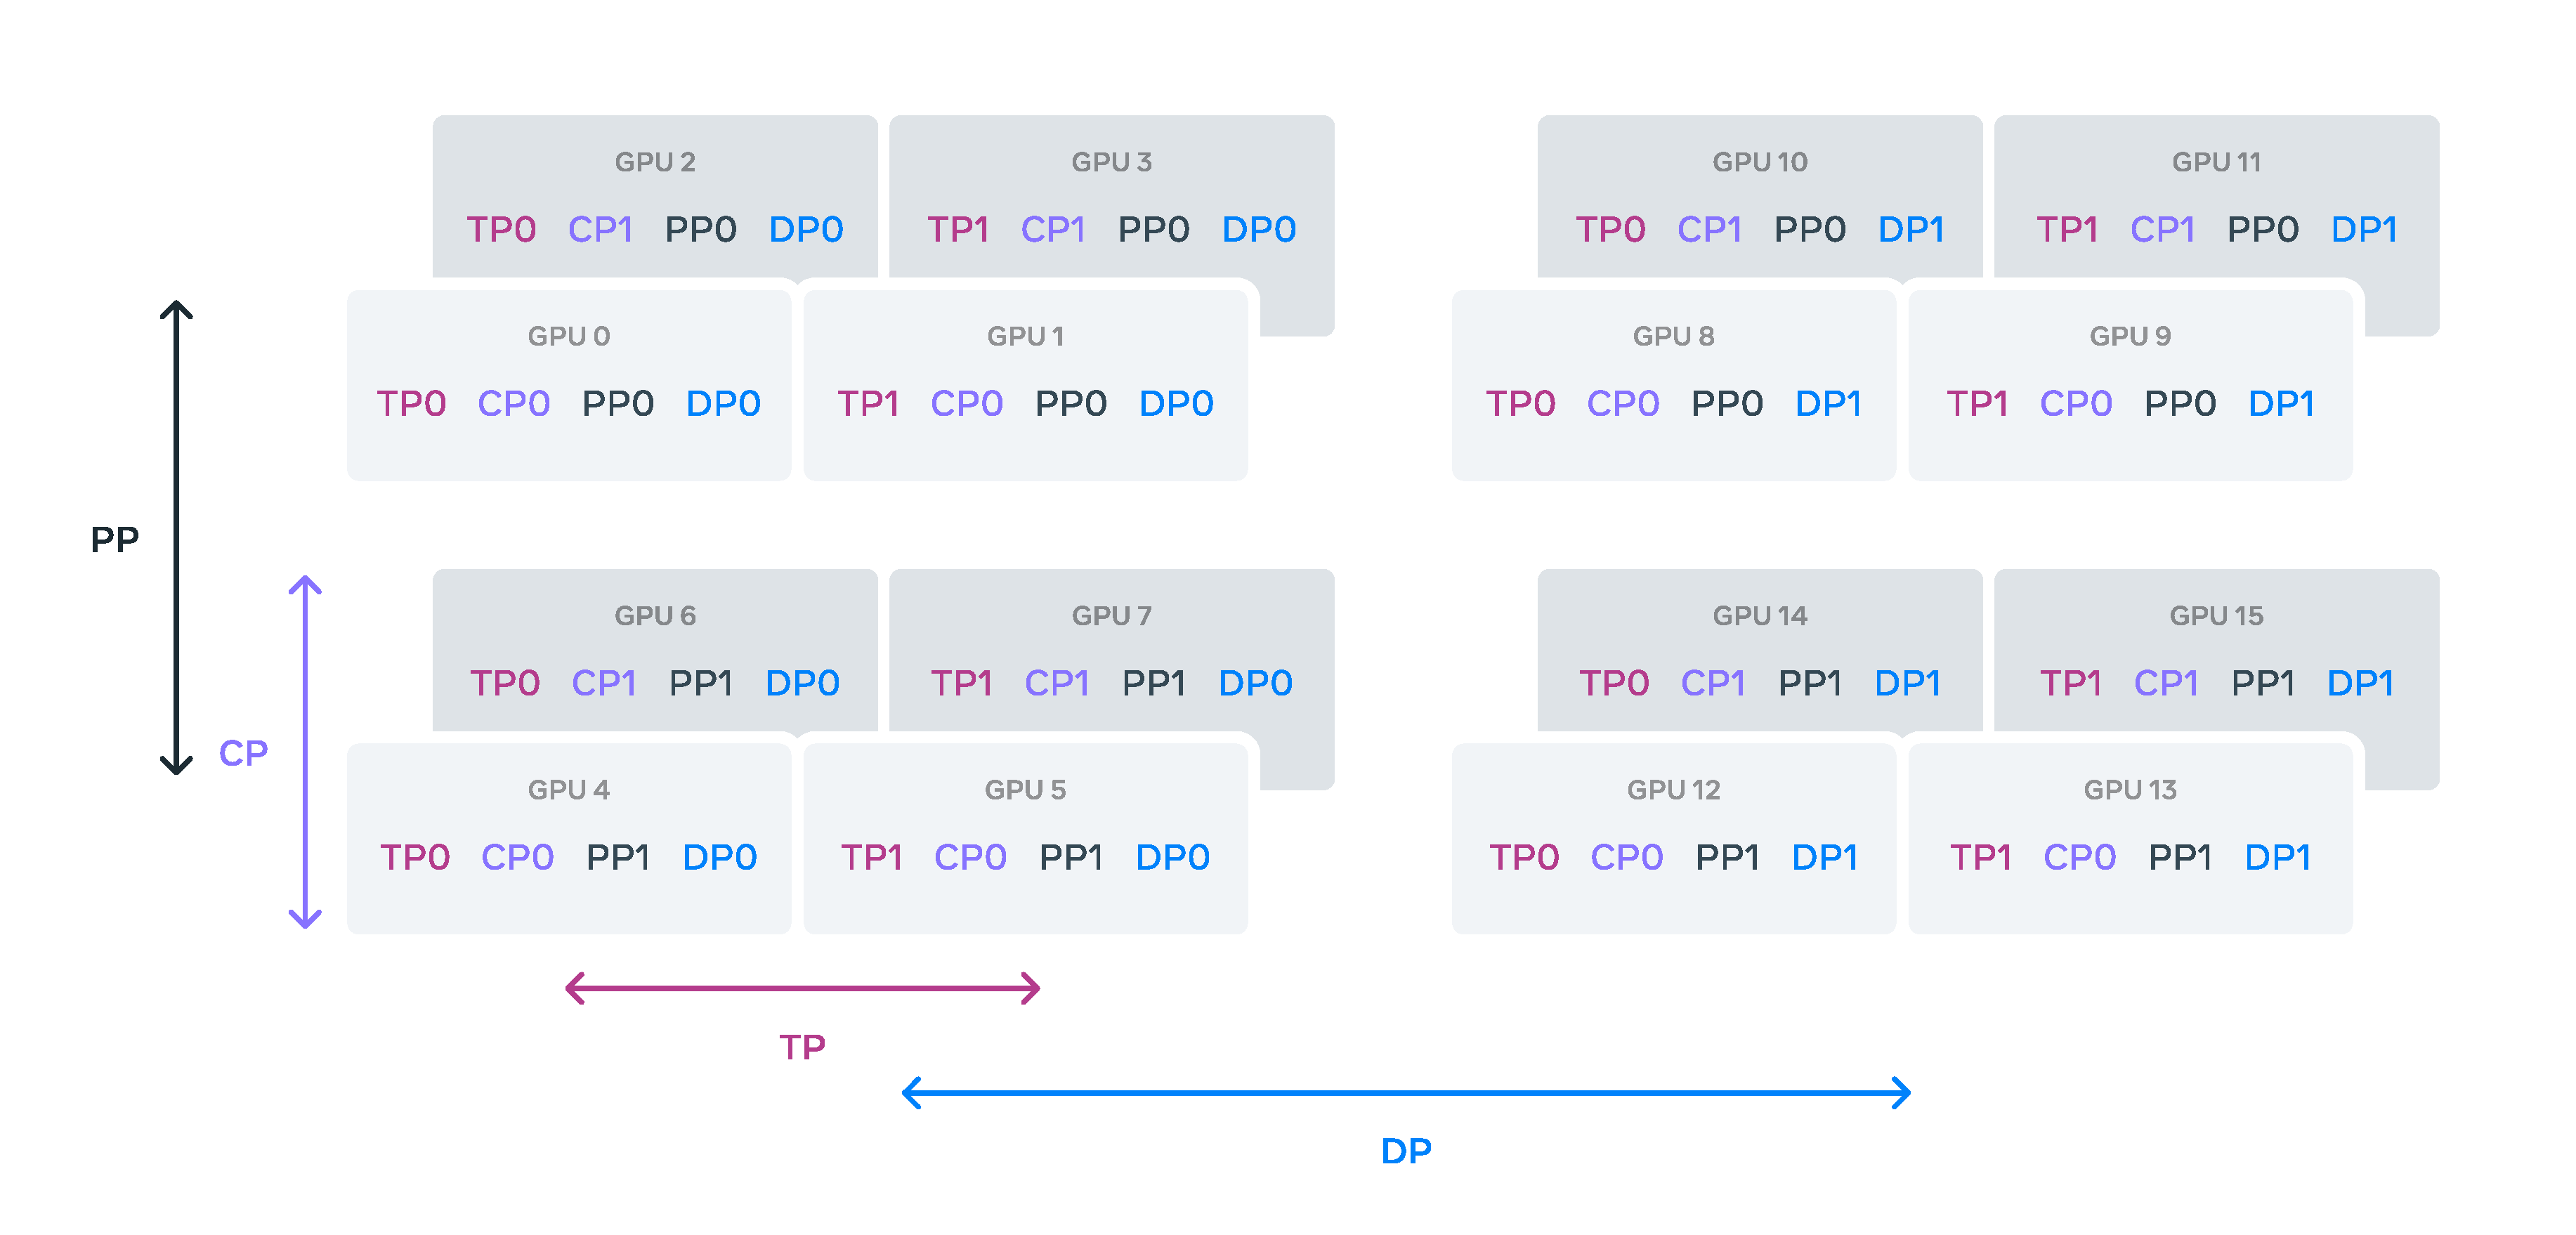
\includegraphics[width=\textwidth]{assets/4D_parallelism.pdf}
     \caption{\textbf{Illustration of 4D parallelism.} GPUs are divided into parallelism groups in the order of [TP, CP, PP, DP], where DP stands for FSDP. In this example, 16 GPUs are configured with a group size of |TP|=2, |CP|=2, |PP|=2, and |DP|=2. 
     A GPU's position in 4D parallelism is represented as a vector, [$D_1$, $D_2$, $D_3$, $D_4$], where $D_i$ is the index on the $i$-th parallelism dimension. In this example,
     GPU0[TP0, CP0, PP0, DP0] and GPU1[TP1, CP0, PP0, DP0] are in the same TP group, GPU0 and GPU2 are in the same CP group, GPU0 and GPU4 are in the same PP group, and GPU0 and GPU8 are in the same DP group.
     }
     \label{fig:4d_parallelism}
\end{figure}

\textbf{Pipeline parallelism improvements.}
We encountered several challenges with existing implementations:

\begin{itemize}
    \item \textbf{Batch size constraint.} Current implementations have constraints on supported batch size per GPU, requiring it to be divisible by the number of pipeline stages. For the example in Figure~\ref{fig:pipeline_parallelism}, the depth-first schedule (DFS) of pipeline parallelism~\citep{narayanan2021efficient} requires $N=\textrm{PP}=4$, while the breadth-first schedule (BFS; \citet{lamy2023breadth}) requires $N=M$, where $M$ is the total number of micro-batches and $N$ is the number of contiguous micro-batches for the same stage's forward or backward. However, pre-training often needs flexibility to adjust batch size.
    
    \item \textbf{Memory imbalance.} Existing pipeline parallelism implementations lead to imbalanced resource consumption. The first stage consumes more memory due to the embedding and the warm-up micro-batches.
    
    \item \textbf{Computation imbalance.} After the last layer of the model, we need to calculate output and loss, making this stage the execution latency bottleneck.
\end{itemize} 

To address these issues, we modify our pipeline schedule as shown in Figure~\ref{fig:pipeline_parallelism}, which allows setting $N$ flexibly---in this case $N=5$, which can run a arbitrary number of micro-batches in each batch. This allows us to run: (1) fewer micro-batches than the number of stages when we have batch size limit at large scale; or (2) more micro-batches to hide point-to-point communication, finding a sweet spot between DFS and breadth first schedule (BFS) for the best communication and memory efficiency. To balance the pipeline, we reduce one Transformer layer each from the first and the last stages, respectively. This means that the first model chunk on the first stage has only the embedding, and the last model chunk on the last stage has only output projection and loss calculation. To reduce pipeline bubbles, we use an interleaved schedule \citep{narayanan2021efficient} with $V$ pipeline stages on one pipeline rank. Overall pipeline bubble ratio is $\frac{\textrm{PP} - 1}{V * M}$. Further, we adopt asynchronous point-to-point communication in PP, which considerably speeds up training, especially in cases when the document mask introduces extra computation imbalance. We enable {\small \texttt{TORCH\_NCCL\_AVOID\_RECORD\_STREAMS}} to reduce memory usage from asynchronous point-to-point communication. Finally, to reduce memory cost, based on detailed memory allocation profiling, we proactively deallocate tensors that will not be used for future computation, including the input and output tensors of each pipeline stage, that will not be used for future computation. With these optimizations, we could pre-train \llamathree on sequences of 8K tokens without activation checkpointing.

\begin{figure*}[t]
     \centering
     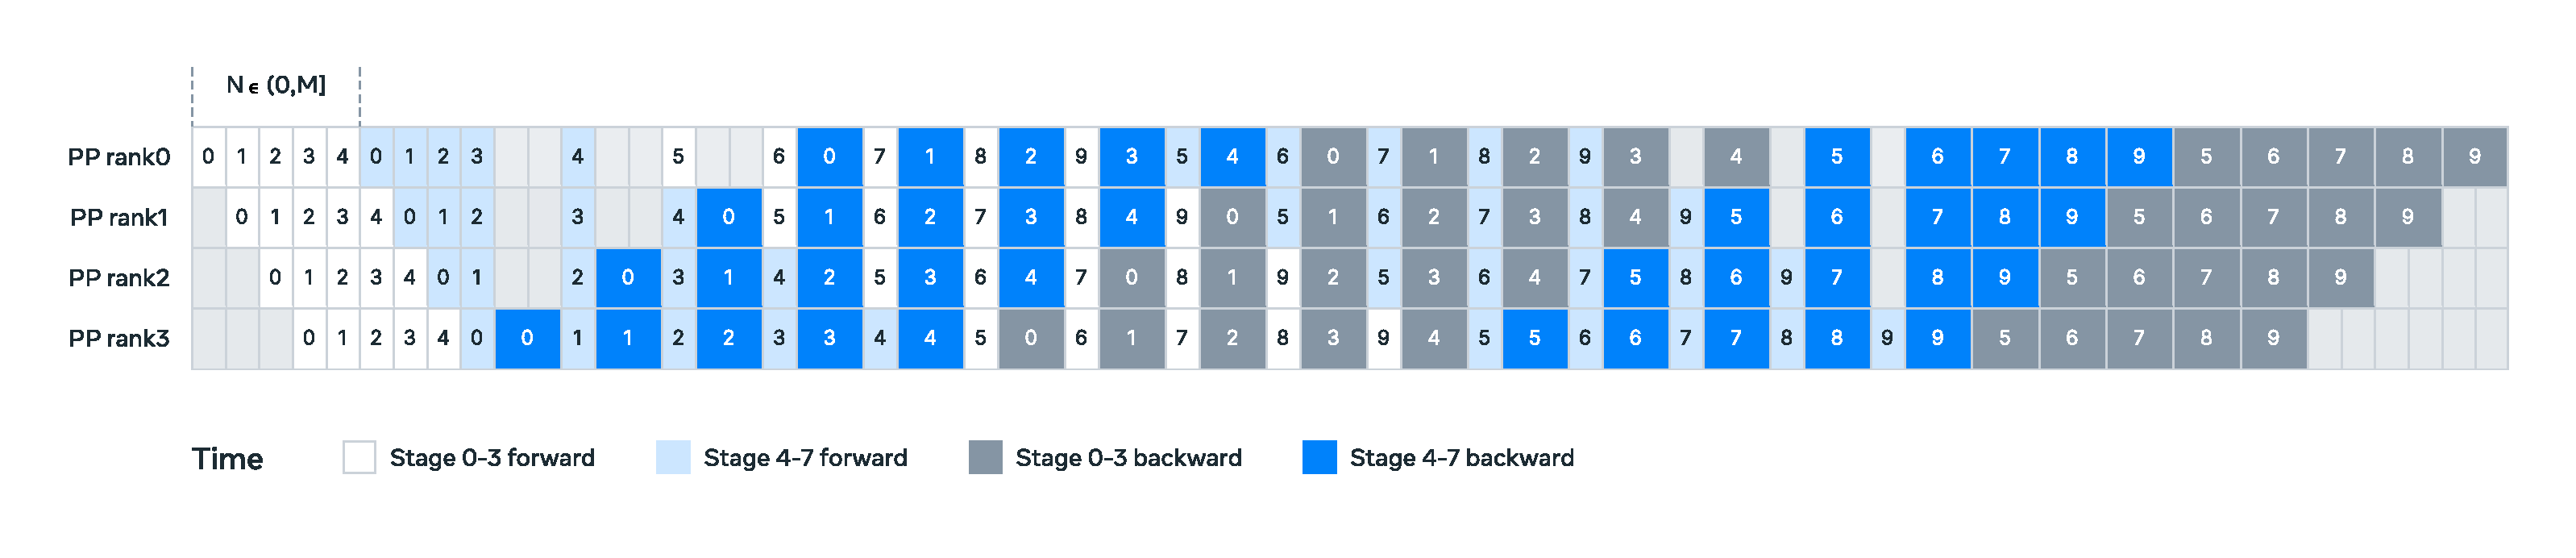
\includegraphics[width=\textwidth]{assets/pipeline_parallelism.pdf}
     \caption{\textbf{Illustration of pipeline parallelism in Llama 3.} Pipeline parallelism partitions eight pipeline stages (0 to 7) across four pipeline ranks (PP ranks 0 to 3), where the GPUs with rank 0 run stages 0 and 4, the GPUs with P rank 1 run stages 1 and 5, \emph{etc}. The colored blocks (0 to 9) represent a sequence of micro-batches, where $M$ is the total number of micro-batches and $N$ is the number of continuous micro-batches for the same stage's forward or backward. Our key insight is to make $N$ tunable.
     }
     \label{fig:pipeline_parallelism}
\end{figure*}

\textbf{Context parallelism for long sequences.} We utilize context parallelism (CP) to improve memory efficiency when scaling the context length of \llamathree and enable training on extremely long sequences up to 128K in length. In CP, we partition across the sequence dimension, and specifically we partition the input sequence into $2 \times \mbox{CP}$ chunks so each CP rank receives two chunks for better load balancing. The $i$-th CP rank received both the $i$-th and the $(2 \times \mbox{CP} - 1 - i)$-th chunks. 

Different from existing CP implementations that overlap communication and computation in a ring-like structure~\citep{liu2023ring}, our CP implementation adopts an \texttt{all-gather} based method where we first \texttt{all-gather} the key (K) and value (V) tensors, and then compute attention output for the local query (Q) tensor chunk. Although the \texttt{all-gather} communication latency is exposed in the critical path, we still adopt this approach for two main reasons: (1) it is easier and more flexible to support different types of attention masks in \texttt{all-gather} based CP attention, such as the document mask; and (2) the exposed \texttt{all-gather} latency is small as the communicated K and V tensors are much smaller than Q tensor due to the use of GQA \citep{ainslie2023gqa}. Hence, the time complexity of attention computation is an order of magnitude larger than \texttt{all-gather} ($O(S^2)$ versus $O(S)$, where $S$ represents the sequence length in the full causal mask), making the \texttt{all-gather} overhead negligible.

\textbf{Network-aware parallelism configuration.} The order of parallelism dimensions, [TP, CP, PP, DP], is optimized for network communication. The innermost parallelism requires the highest network bandwidth and lowest latency, and hence is usually constrained to within the same server. The outermost parallelism may spread across a multi-hop network and should tolerate higher network latency. Therefore, based on the requirements for network bandwidth and latency, we place parallelism dimensions in the order of [TP, CP, PP, DP]. DP (\emph{i.e.}, FSDP) is the outermost parallelism because it can tolerate longer network latency by asynchronously prefetching sharded model weights and reducing gradients. Identifying the optimal parallelism configuration with minimal communication overhead while avoiding GPU memory overflow is challenging. We develop a memory consumption estimator and a performance-projection tool which helped us explore various parallelism configurations and project overall training performance and identify memory gaps effectively.

\textbf{Numerical stability.} By comparing training loss between different parallelism setups, we fixed several numerical issues that impact training stability. To ensure training convergence, we use FP32 gradient accumulation during backward computation over multiple micro-batches and also \texttt{reduce-scatter} gradients in FP32 across data parallel workers in FSDP. For intermediate tensors, \emph{e.g.}, vision encoder outputs, that are used multiple times in the forward computation, the backward gradients are also accumulated in FP32.

\subsubsection{Collective Communication}
\label{sec:ncclx}

Our collective communication library for \llamathree is based on a fork of Nvidia's NCCL library, called NCCLX. NCCLX significantly improves the performance of NCCL, especially for higher latency networks. Recall that the order of parallelism dimensions is [TP, CP, PP, DP], where DP corresponds to FSDP. The outermost parallelism dimensions, PP and DP, may communicate through a multi-hop network, with latency up to tens of microseconds. The original NCCL collectives---\texttt{all-gather} and \texttt{reduce-scatter} in FSDP, and \texttt{point-to-point} in PP---require data chunking and staged data copy. This approach incurs several inefficiencies, including (1) requiring a large number of small control messages to be exchanged over the network to facilitate data transfer, (2) extra memory-copy operations, and (3) using extra GPU cycles for communication.  For \llamathree training, we address a subset of these inefficiencies by tuning chunking and data transfer to fit our network latencies, which can be as high as tens of microseconds for a large cluster. We also allow small control messages to traverse our network at a higher priority, especially avoiding being head-of-line blocked in deep-buffer core switches. Our ongoing work for future Llama versions involves making deeper changes in NCCLX to holistically address all the aforementioned problems.

\subsubsection{Reliability and Operational Challenges}

The complexity and potential failure scenarios of 16K GPU training surpass those of much larger CPU clusters that we have operated. Moreover, the synchronous nature of training makes it less fault-tolerant---a single GPU failure may require a restart of the entire job. Despite these challenges, for \llamathree, we achieved higher than 90\% effective training time while supporting automated cluster maintenance, such as firmware and Linux kernel upgrades~\citep{leonhardi2024maintenance}, which resulted in at least one~training interruption daily. The effective training time measures the time spent on useful training over the elapsed time.

During a 54-day snapshot period of pre-training, we experienced a total of 466 job interruptions. Of these, 47 were planned interruptions due to automated maintenance operations such as firmware upgrades or operator-initiated operations like configuration or dataset updates. The remaining 419 were unexpected interruptions, which are classified in Table~\ref{table:job_interruptions}.
Approximately 78\% of the unexpected interruptions are attributed to confirmed hardware issues, such as GPU or host component failures, or suspected hardware-related issues like silent data corruption and unplanned individual host maintenance events. GPU issues are the largest category, accounting for 58.7\% of all unexpected issues.  Despite the large number of failures, significant manual intervention was required only three times during this period, with the rest of issues handled by automation. 

\begin{table}[]
\centering
\begin{tabular}{lccc}
    \toprule
\textbf{Component}             & \textbf{Category} & \textbf{Interruption Count} & \textbf{\% of Interruptions} \\
\midrule
Faulty GPU                            & GPU               & 148                         & 30.1\%                       \\
GPU HBM3 Memory                & GPU               & 72                          & 17.2\%                       \\
Software Bug                   & Dependency          & 54                          & 12.9\%                       \\
Network Switch/Cable           & Network           & 35                          & 8.4\%                        \\
Host Maintenance               & \begin{tabular}[c]{@{}c@{}}Unplanned \\ Maintenance\end{tabular}       & 32                          & 7.6\%                        \\
GPU SRAM Memory                & GPU               & 19                          & 4.5\%                        \\
GPU System Processor           & GPU               & 17                          & 4.1\%                        \\
NIC                            & Host              & 7                           & 1.7\%                        \\
NCCL Watchdog Timeouts                  & Unknown           & 7                           & 1.7\%                        \\
Silent Data Corruption                      & GPU           & 6                           & 1.4\%                        \\
GPU Thermal Interface + Sensor & GPU               & 6                           & 1.4\%                        \\
SSD                            & Host              & 3                           & 0.7\%                        \\
Power Supply                   & Host              & 3                           & 0.7\%                        \\
Server Chassis                 & Host              & 2                           & 0.5\%                        \\
IO Expansion Board             & Host              & 2                           & 0.5\%                        \\
Dependency                     & Dependency        & 2                           & 0.5\%                        \\
CPU                            & Host              & 2                           & 0.5\%                        \\
System Memory                  & Host              & 2                           & 0.5\%    \\
\bottomrule
\end{tabular}
\caption{\textbf{Root-cause categorization of unexpected interruptions during a 54-day period of Llama 3 405B pre-training.} About 78\% of unexpected interruptions were attributed to confirmed or suspected hardware issues. }
\label{table:job_interruptions}
\end{table}

To increase the effective training time, we reduced job startup and checkpointing time, and developed tools for fast diagnosis and problem resolution. We extensively use PyTorch's built-in NCCL flight recorder~\citep{ansel2024pytorch}, a feature that captures collective metadata and stack traces into a ring buffer, and hence allowing us to diagnose hangs and performance issues quickly at scale, particularly with regard to NCCLX. Using this, we efficiently record every communication event and the duration of each collective operation, and also automatically dump tracing data on NCCLX watchdog or heartbeat timeout. We enable more computationally intensive tracing operations and metadata collection selectively as needed live in production through online configuration changes~\citep{configerator} without needing a code release or job restart.

Debugging issues in large-scale training is complicated by the mixed use of NVLink and RoCE in our network. Data transfer over NVLink typically occurs through load/store operations issued by CUDA kernels, and failures in either the remote GPU or NVLink connectivity often manifest as stalled load/store operations within CUDA kernels without returning a clear error code. NCCLX enhances the speed and accuracy of failure detection and localization through a tight co-design with PyTorch, allowing PyTorch to access NCCLX’s internal state and track relevant information. While stalls due to NVLink failures cannot be completely prevented, our system monitors the state of the communication library and automatically times out when such a stall is detected. Additionally, NCCLX traces the kernel and network activities of each NCCLX communication and provides a snapshot of the failing NCCLX collective's internal state, including finished and pending data transfers between all ranks. We analyze this data to debug NCCLX scaling issues.

Sometimes, hardware issues may cause still-functioning but slow stragglers that are hard to detect. Even a single straggler can slow down thousands of other GPUs, often appearing as functioning but slow communications. We developed tools to prioritize potentially problematic communications from selected process groups. By investigating just a few top suspects,  we were usually able to effectively identify the stragglers.

One interesting observation is the impact of environmental factors on training performance at scale. For Llama 3 405B , we noted a diurnal 1-2\% throughput variation based on time-of-day. This fluctuation is the result of higher mid-day temperatures impacting GPU dynamic voltage and frequency scaling.

During training, tens of thousands of GPUs may increase or decrease power consumption at the same time, for example, due to all GPUs waiting for checkpointing or collective communications to finish, or the startup or shutdown of the entire training job. When this happens, it can result in instant fluctuations of power consumption across the data center on the order of tens of megawatts, stretching the limits of the power grid. This is an ongoing challenge for us as we scale training for future, even larger Llama models.

\subsection{Pre-training}
\label{section:vision_training_recipe}

\textbf{Image.}
We initialize from the pre-trained text model and vision encoder weights.
The vision encoder is unfrozen, while the text model weights are kept frozen as explained above.
First, we train the model using 6B image-text pairs where each image is resized to fit within four tiles of $336 \times 336$ pixels.
We use a global batch size of 16,384 and a cosine learning rate schedule with initial learning rate $10 \times 10^{-4}$ and a weight decay of $0.01$.
The initial learning rate was determined based on small-scale experiments.
However,  these findings did not generalize well to very long training schedules and dropped the learning rate a few times during training when the loss values became stagnant.
After the base pre-training, we increase the image resolution further and continue training the same weights on the annealing dataset.
The optimizer is re-initialized via warm-up to learning rate $2 \times 10^{-5}$ and again follows a cosine schedule.

\textbf{Video.}
For video pre-training, we start from the image pre-trained and annealed weights as described above.
We add the video aggregator and cross-attention layers as described in the architecture, initialized randomly. We freeze all the parameters in the model except the video-specific ones (the aggregator and video cross-attention), and train them on the video pre-training data.
We use the same training hyperparameters as the image annealing stage, with small differences in the learning rate.
We uniformly sample 16 frames from the full video, and represent each frame using four chunks, each of size of $448 \times 448$ pixels.
We use an aggregation factor of 16 in the video aggregator, hence obtaining one effective frame, which the text tokens cross-attend to.
We use a global batch size of 4,096, a sequence length of 190 tokens, and a learning rate of $10^{-4}$ during training.

\subsection{Post-Training}
\label{section:vision_post_training}
In this section, we describe the post-training recipe for our vision adapters. After pre-training, we fine-tune the model on highly curated multi-modal conversational data to enable chat capabilities. We further implement direct preference optimization (DPO) to boost human evaluation performance and rejection sampling to improve multi-modal reasoning capabilities. Finally, we add a quality-tuning stage where we continue fine-tuning the model on a very small set of high-quality conversational data which further boosts human evaluation while retaining performance across benchmarks. More details on each of these steps are provided below.

\subsubsection{Supervised Finetuning Data}
\label{subsubsection:vision_supervised_finetuning_data}
We describe our supervised finetuning (SFT) data for image and video capabilities separately below.

\textbf{Image.} We utilize a mix of different datasets for supervised finetuning.
\begin{itemize}
\item \textbf{Academic datasets.} We convert a highly filtered collection of existing academic datasets to question-answer pairs using templates or via LLM rewriting. The LLM rewriting's purpose is to augment the data with different instructions and to improve the language quality of answers.

\item \textbf{Human annotations.} We collect multi-modal conversation data via human annotators for a wide range of tasks (open-ended question-answering, captioning, practical use cases, \textit{etc.}) and domains (\textit{e.g.}, natural images and structured images). Annotators are provided with images and asked to write conversations. To ensure diversity, we cluster large-scale datasets and sampled images uniformly across different clusters. Further, we acquire additional images for a few specific domains by expanding a seed via k-nearest neighbors. Annotators are also provided with intermediate checkpoints of existing models to facilitate model-in-the-loop style annotations, so that model generations can be utilized as a starting point by the annotators to then provide additional human edits. This is an iterative process, in which model checkpoints would be regularly updated with better performing versions trained on the latest data. This increases the volume and efficiency of human annotations, while also improving their quality.

\item \textbf{Synthetic data.} We explore different ways to generate synthetic multi-modal data by using text-representations of images and a text-input LLM. The high-level idea is to utilize the reasoning capabilities of text-input LLMs to generate question-answer pairs in the text domain, and replace the text representation with its corresponding images to produce synthetic multi-modal data. Examples include rendering texts from question-answer datasets as images or rendering table data into synthetic images of tables and charts. Additionally, we use captions and OCR extractions from existing images to generate additional conversational or question-answer data related to the images.
\end{itemize}

\textbf{Video.} Similar to the image adapter, we use academic datasets with pre-existing annotations and convert them into appropriate textual instructions and target responses.
The targets are converted to open-ended responses or multiple-choice options, whichever is more appropriate.
We ask humans to annotate videos with questions and corresponding answers.
The annotators are asked to focus on questions that could not be answered based on a single frame, to steer the annotators towards questions that require temporal understanding.

\subsubsection{Supervised Finetuning Recipe}
We describe our supervised finetuning (SFT) recipe for image and video capabilities separately below.

\label{subsubsection:vision_supervised_finetuning_recipe}
\textbf{Image.} We initialize from the pre-trained image adapter, but hot-swap the pre-trained language model's weights with the instruction tuned language model's weights. The language model weights are kept frozen to maintain text-only performance, \textit{i.e.}, we only update the vision encoder and image adapter weights.

Our approach to finetune the model is similar to \cite{wortsman2022modelsoupsaveragingweights}. First, we run a hyperparameter sweep using multiple random subsets of data, learning rates and weight decay values. Next, we rank the models based on their performance. Finally, we average the weights of the top-$K$ models to obtain the final model. The value of $K$ is determined by evaluating the averaged models and selecting the instance with highest performance. We observe that the averaged models consistently yield better results compared to the best individual model found via grid search. Further, this strategy reduces sensitivity to hyperparameters.

\textbf{Video.} For video SFT, we initialize the video aggregator and cross-attention layers using the pre-trained weights.
The rest of the parameters in the model, the image weights and the LLM, are initialized from corresponding models following their finetuning stages.
Similar to video pre-training, we then finetune only the video parameters on the video SFT data.
For this stage, we increase the video length to 64 frames, and use an aggregation factor of 32 to get two effective frames.
The resolution of the chunks is also increased to be consistent with the corresponding image hyperparameters.

\subsubsection{Preference Data}
\label{subsubsection:vision_preference_data}
We built multimodal pair-wise preference datasets for reward modeling and direct preference optimization.
\begin{itemize}

\item \textbf{Human annotations.} The human-annotated preference data consists of comparisons between two different model outputs, labeled as ``chosen'' and ``rejected'', with 7-scale ratings. The models used to generate responses are sampled on-the-fly from a pool of the best recent models, each with different characteristics. We update the model pool weekly. Besides preference labels, we also request annotators to provide optional human edits to correct inaccuracies in ``chosen'' responses because vision tasks have a low tolerance for inaccuracies. Note that human editing is an optional step because there is a trade-off between volume and quality in practice.

\item \textbf{Synthetic data.} Synthetic preference pairs could also be generated by using text-only LLMs to edit and deliberately introduce errors in the supervised finetuning dataset. We took the conversational data as input, and use an LLM to introduce subtle but meaningful errors (\textit{e.g.}, change objects, change attributes, add mistakes in calculations, etc.). These edited responses are used as negative ``rejected'' samples and paired with the ``chosen'' original supervised finetuning data.

\item \textbf{Rejection sampling.} Furthermore, to create more \emph{on-policy} negative samples, we leveraged the iterative process of rejection sampling to collect additional preference data. We discuss our usage of rejection sampling in more detail in the following sections. At a high-level, rejection sampling is used to iteratively sample high-quality generations from a model. Therefore, as a by-product, all generations that are not selected can be used as negative rejected samples and used as additional preference data pairs.

\end{itemize}

\subsubsection{Reward Modeling}
\label{subsubsection:vision_reward_modeling}
We train a vision reward model (RM) on top of the vision SFT model and the language RM. The vision encoder and the cross-attention layers are initialized from the vision SFT model and unfrozen during training, while the self-attention layers are initialized from the language RM and kept frozen. We observe that freezing the language RM part generally leads to better accuracy, especially on tasks that require the RM to judge based on its knowledge or the language quality. We adopt the same training objective as the language RM, but adding a weighted regularization term on the square of the reward logits averaged over the batch, which prevents the reward scores from drifting.

The human preference annotations in Section~\ref{subsubsection:vision_preference_data} are used to train the vision RM. We follow the same practice as language preference data (Section~\ref{sec:rlhf_annotation_data}) to create two or three pairs with clear ranking (\emph{edited} > \emph{chosen} > \emph{rejected}). In addition, we also synthetically augment the negative responses by perturbing the words or phrases related to the information in the image (such as numbers or visual texts). This encourages the vision RM to ground its judgement based on the actual image content.

\subsubsection{Direct Preference Optimization}
\label{subsubsec:dpo}
Similar to the language model (Section~\ref{subsubsec:postdpo}), we further train the vision adapters with Direct Preference Optimization (DPO;~\cite{rafailov2023dpo}) using the preference data described in Section~\ref{subsubsection:vision_preference_data}. To combat the distribution shift during post-training rounds, we only keep recent batches of human preference annotations while dropping batches that are sufficiently off-policy (\textit{e.g.}, if the base pre-trained model is changed). We find that instead of always freezing the reference model, updating it in an exponential moving average (EMA) fashion every k-steps helps the model learn more from the data, resulting in better performance in human evaluations. Overall, we observed that the vision DPO model consistently performs better than its SFT starting point in human evaluations for every finetuning iteration.

\subsubsection{Rejection Sampling}
\label{subsubsection:vision_rejection_sampling}
Most available question-answer pairs only contain the final answer and lack the chain-of-thought explanation that is required to train a model that generalizes well for reasoning tasks.
We use rejection sampling to generate the missing explanations for such examples and boost the model's reasoning capabilities.

Given a question-answer pair, we generate multiple answers by sampling the finetuned model with different system prompts or temperature.
Next, we compare the generated answers to the ground-truth via heuristics or an LLM judge.
Finally, we retrain the model by adding the correct answers back into the finetuning data mix. We find it useful to keep multiple correct answers per question.

To ensure we only add high-quality examples back into training, we implemented the following two guardrails.
First, we find that some examples contain incorrect explanations, despite the final answer being correct.
We observed that this pattern occurs more frequently for questions where only a small fraction of the generated answers is correct.
Therefore, we drop answers for questions where the probability of the answer being correct is below a certain threshold.
Second, raters prefer some answers over others due to differences in language or style.
We use the reward model to select top-$K$ highest-quality answers and add them back into training.

\subsubsection{Quality Tuning}
\label{subsubsection:vision_quality_tuning}
We curate a small but \emph{highly} selective SFT dataset where all samples have been rewritten and verified either by humans or our best models to meet our highest standards. We train DPO models with this data to improve response quality, calling the process Quality-Tuning (QT). We find that QT significantly improves human evaluations without affecting generalization verified by benchmarks when the QT dataset covers a wide range of tasks and proper early stopping is applied. We select checkpoints at this stage purely based on benchmarks to ensure capabilities are retained or improved.

\begin{NiceTabular}{lccccccc}
    \CodeBefore
    \Body
    \toprule
    & \textbf{Llama 3-V 8B} & \textbf{Llama 3-V 70B} & \textbf{Llama 3-V 405B} & \textbf{GPT-4V} & \textbf{GPT-4o} & \textbf{Gemini 1.5 Pro} & \textbf{Claude 3.5} \\
    \midrule
    MMMU \scriptsize{(val, CoT)} & 49.6 & 60.6 & 64.5 & 56.4 & \textbf{69.1} & 62.2 & 68.3 \\
    VQAv2 \scriptsize{(test-dev)} & 78.0 & 79.1 & \textbf{80.2} & 77.2 & -- & \textbf{80.2} & --\\
    AI2 Diagram \scriptsize{(test)} & 84.4 & 93.0 & 94.1 & 78.2 & 94.2 & 94.4 & \textbf{94.7} \\
    ChartQA \scriptsize{(test, CoT)} & 78.7 & 83.2 & 85.8 & 78.4 & 85.7 & 87.2 & \textbf{90.8} \\
    TextVQA \scriptsize{(val)} & 78.2 & 83.4 & \textbf{84.8} & 78.0 & -- & 78.7 & --\\
    DocVQA \scriptsize{(test)} & 84.4 & 92.2 & 92.6 & 88.4 & 92.8 & ~~93.1$^{\triangle}$ & \textbf{95.2} \\
    \bottomrule
\end{NiceTabular}

\begin{NiceTabular}{lccccccc}
    \CodeBefore
    \Body
    \toprule
    & \textbf{Llama 3-V 8B} & \textbf{Llama 3-V 70B} & \textbf{Gemini 1.0 Pro} & \textbf{Gemini 1.0 Ultra} & \textbf{Gemini 1.5 Pro} & \textbf{GPT-4V} & \textbf{GPT-4o} \\
    \midrule
    PerceptionTest \scriptsize{(test)} & 53.8 & \textbf{60.8} & 51.1 & 54.7 & -- & -- & -- \\
    TVQA \scriptsize{(val)} & 82.5 & \textbf{87.9} & -- & -- & -- & 87.3 & -- \\
    NExT-QA \scriptsize{(test)} & 27.3 & \textbf{30.3} & 28.0 & 29.9 & -- & -- & -- \\
    ActivityNet-QA \scriptsize{(test)} & 52.7 & 56.3 & 49.8 & 52.2 & 57.5 & -- & \textbf{61.9} \\
    \bottomrule
\end{NiceTabular}

